%LTeX: language=it
\subsection{UC 8 - Modificare un contatto} \label{sec:UC8}
    \begin{itemize}
        \item \textbf{Attore principale}: MUA;
        \item \textbf{Descrizione}: il MUA deve poter modificare un contato nel sistema;
        \item \textbf{Precondizioni}: l’account che il MUA gestisce è registrato nel sistema, e ha un connessione aperta con il sistema ed è autenticato;
        \item \textbf{Postcondizioni}: il MUA modifica un contatto, il suo nuovo stato viene salvato nel sistema;
        \item \textbf{Scenario principale}:
            \begin{enumerate}
                \item il MUA invia le informazioni per aggiornare il contatto nel sistema (\hyperref[sec:UC8.1]{UC 8.1});
                \item il sistema salva il nuovo stato del contato;
            \end{enumerate}
        \item \textbf{Inclusioni}: nessuna;
        \item \textbf{Generalizzazioni}: nessuna;
        \item \textbf{Estensioni}: nessuna.
    \end{itemize}

\begin{figure}[h]
    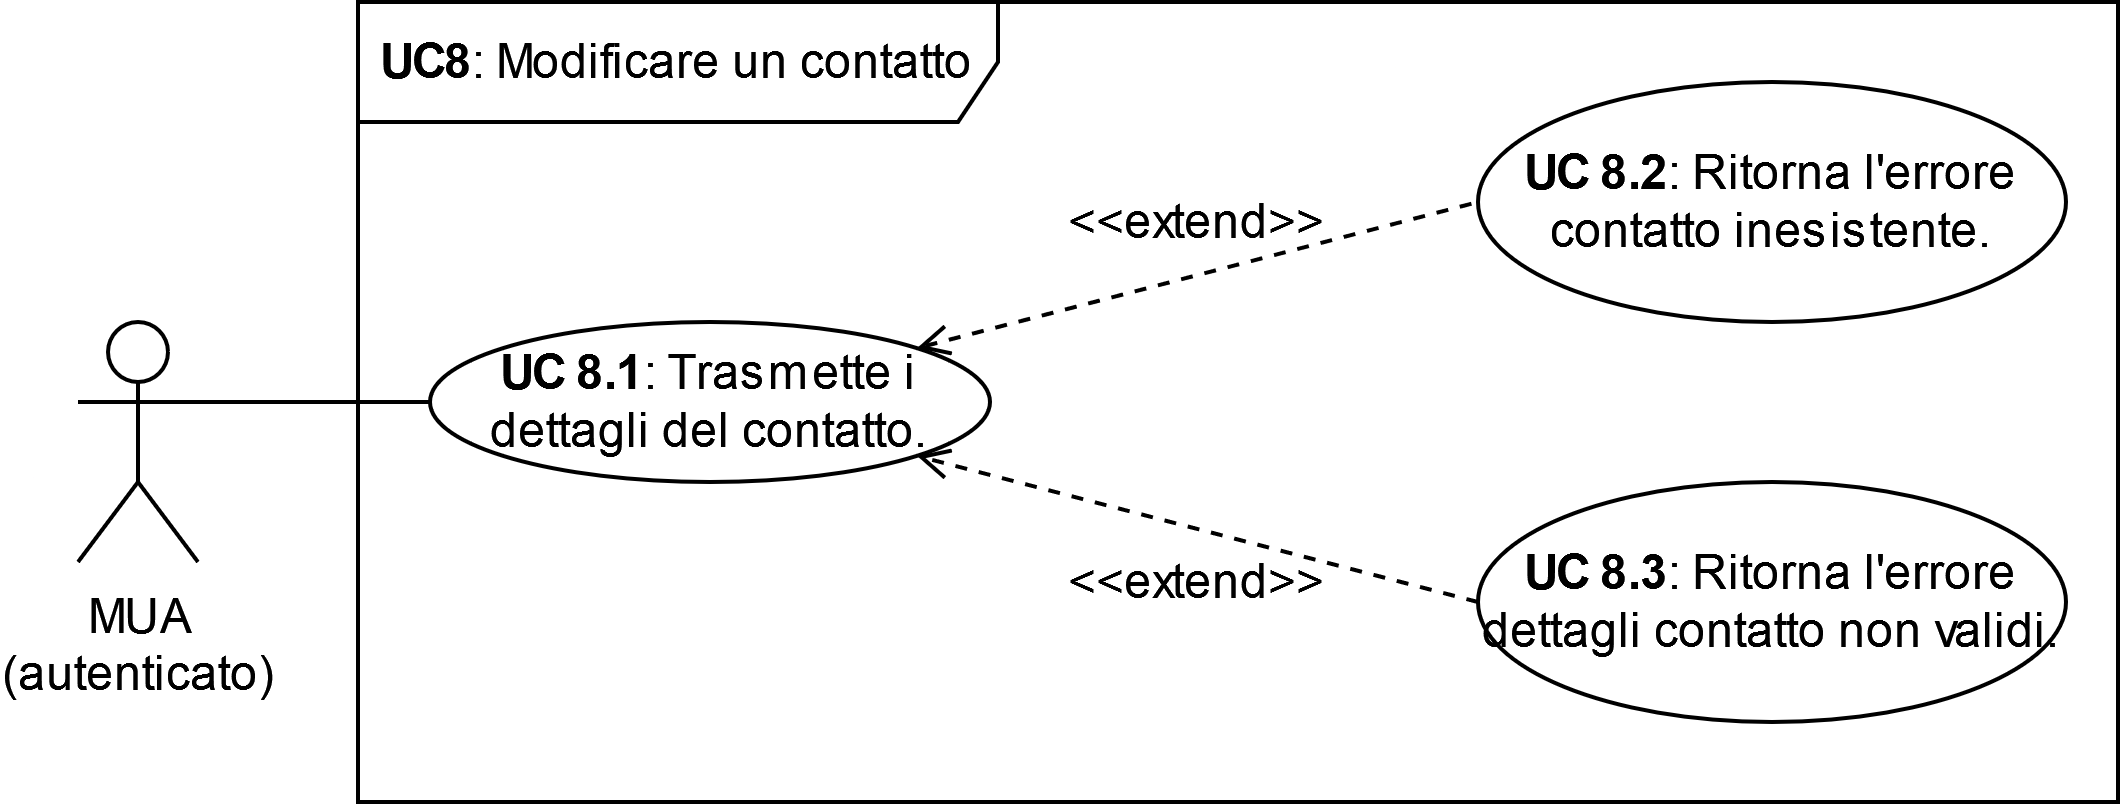
\includegraphics[width=0.85\textwidth]{sections/uc_imgs/UC08.X.png}
    \centering
    \caption{Diagramma sotto-casi UC 8.}
\end{figure}

\subsubsection{UC 8.1 - Trasmette i dettagli del contatto} \label{sec:UC8.1}
    \begin{itemize}
        \item \textbf{Attore principale}: MUA;
        \item \textbf{Descrizione}: il MUA trasmette il nuovo stato del contato al sistema;
        \item \textbf{Precondizioni}: il MUA sta utilizzando la funzionalità di modifica di un contatto;
        \item \textbf{Postcondizioni}: il MUA modifica un contatto, il suo nuovo stato viene salvato nel sistema;
        \item \textbf{Scenario principale}:
            \begin{enumerate}
                \item il MUA invia le informazioni per aggiornare il contatto nel sistema;
                \item il sistema elabora le nuove informazioni, e controlla che siano valide;
                \item il sistema salva il nuovo stato del contato;
            \end{enumerate}
        \item \textbf{Inclusioni}: nessuna;
        \item \textbf{Generalizzazioni}: nessuna;
        \item \textbf{Estensioni}: 
            \begin{enumerate}[label=\alph*.]
                \item il sistema non riesce ad aggiornare lo stato del contato perché non è stato trovato:
                \begin{enumerate}[label=\arabic*.]
                    \item il sistema ritorna un errore al MUA di contatto inesistente (\hyperref[sec:UC8.2]{UC 8.2});
                \end{enumerate}
                \item il sistema non riesce a modificare lo stato del contato perché i dati trasmessi non rispettano i requisiti:
                \begin{enumerate}[label=\arabic*.]
                    \item il sistema ritorna un errore al MUA dettagli contatto non validi (\hyperref[sec:U8.3]{UC 8.3}).
                \end{enumerate}
            \end{enumerate}
    \end{itemize}

\subsubsection{UC 8.2 - Ritorna l'errore contatto inesistente} \label{sec:UC8.2}
    \begin{itemize}
        \item \textbf{Attore principale}: MUA;
        \item \textbf{Descrizione}: il MUA sta trasmettendo il nuovo stato del contato al sistema, ma il contatto indicato non esiste;
        \item \textbf{Precondizioni}: il MUA sta utilizzando la funzionalità di trasmissione dei dettagli per la modifica di un contatto;
        \item \textbf{Postcondizioni}: il sistema non aggiorna lo stato del contatto, il MUA è stato notificato dell'errore;
        \item \textbf{Scenario principale}:
            \begin{enumerate}
                \item il MUA invia le informazioni per aggiornare il contatto nel sistema;
                \item il sistema controlla le informazioni, e riscontra che il contatto non esiste;
                \item il sistema non aggiorna il contatto;
                \item il sistema ritorna l'errore al MUA;
            \end{enumerate}
        \item \textbf{Inclusioni}: nessuna;
        \item \textbf{Generalizzazioni}: nessuna;
        \item \textbf{Estensioni}: nessuna.
    \end{itemize}

\subsubsection{UC 8.3 - Ritorna l'errore dettagli contatto non validi} \label{sec:UC8.3}
    \begin{itemize}
        \item \textbf{Attore principale}: MUA;
        \item \textbf{Descrizione}: il MUA sta trasmettendo il nuovo stato del contato al sistema, ma i dettagli inviati non rispettano i requisiti richiesti;
        \item \textbf{Precondizioni}: il MUA sta utilizzando la funzionalità di trasmissione dei dettagli per la modifica di un contatto;
        \item \textbf{Postcondizioni}: il sistema non aggiorna lo stato del contatto, il MUA è stato notificato dell'errore;
        \item \textbf{Scenario principale}:
            \begin{enumerate}
                \item il MUA invia le informazioni per aggiornare il contatto nel sistema;
                \item il sistema controlla le informazioni, il sistema riscontra dei valori non validi;
                \item il sistema non aggiorna il contatto;
                \item il sistema ritorna l'errore al MUA;
            \end{enumerate}
        \item \textbf{Inclusioni}: nessuna;
        \item \textbf{Generalizzazioni}: nessuna;
        \item \textbf{Estensioni}: nessuna.
    \end{itemize}